\documentclass[a4paper, 11pt]{article}
\usepackage[cpp,linenum]{mypackage}
\usepackage{float}
\usepackage{amsmath}
\usepackage{graphicx}
\usepackage{geometry}
\usepackage{listings}
\geometry{scale=0.8}
% \linespread{1.5}
\usepackage[colorlinks,linkcolor=red]{hyperref}

\lstset{language=prolog}

\title{	
\normalfont \normalsize
\textsc{School of Data and Computer Science, Sun Yat-sen University} \\ [25pt] %textsc small capital letters
\rule{\textwidth}{0.5pt} \\[0.4cm] % Thin top horizontal rule
\huge  Lab 5 Family Problem (Prolog)\\ % The assignment title
\rule{\textwidth}{2pt} \\[0.5cm] % Thick bottom horizontal rule
\author{17341015 Hongzheng Chen}
\date{\normalsize\today}
}

\begin{document}
\maketitle
\tableofcontents
\newpage

\section{About Cousin and Removed}
\textbf{What Is a First Cousin, Twice Removed?}

If someone walked up to you and said, "Howdy, I'm your third cousin, twice removed," would you have any idea what they meant? Most people have a good understanding of basic relationship words such as "mother," "father," "aunt," "uncle," "brother," and "sister." But what about the relationship terms that we don't use in everyday speech? Terms like "second cousin" and "first cousin, once removed"? We don't tend to speak about our relationships in such exact terms ("cousin" seems good enough when you are introducing one person to another), so most of us aren't familiar with what these words mean.

\textbf{Relationship Terms}

Sometimes, especially when working on your family history, it's handy to know how to describe your family relationships more exactly. The definitions below should help you out.

\textbf{Cousin (a.k.a "first cousin")}

Your first cousins are the people in your family who have two of the same grandparents as you. In other words, they are the children of your aunts and uncles.

\textbf{Second Cousin}

Your second cousins are the people in your family who have the same great-grandparents as you., but not the same grandparents.

\textbf{Third, Fourth, and Fifth Cousins}

Your third cousins have the same great great grandparents, fourth cousins have the same great-great-great-grandparents, and so on.

\textbf{Removed}

When the word "removed" is used to describe a relationship, it indicates that the two people are from different generations. You and your first cousins are in the same generation (two generations younger than your grandparents), so the word "removed" is not used to describe your relationship.

The words "\textbf{once removed}" mean that there is a difference of one generation. For example, your mother's first cousin is your first cousin, once removed. This is because your mother's first cousin is one generation younger than your grandparents and you are two generations younger than your grandparents. This one-generation difference equals "once removed."

\textbf{Twice removed} means that there is a two-generation difference. You are two generations younger than a first cousin of your grandmother, so you and your grandmother's first cousin are first cousins, twice removed.
\section{Problem Description}
Please fulfill the following tasks by using \texttt{Prolog}:
\begin{enumerate}
\item Write sentences describing the predicates \textbf{Grandchild}, \textbf{Greatgrandparent}, \textbf{Ancestor}, \textbf{Brother}, \textbf{Sister}, \textbf{Daughter}, \textbf{Son}, \textbf{FirstCousin}, \textbf{BrotherInLaw}, \textbf{SisterInLaw}, \textbf{Aunt}, and \textbf{Uncle}. \emph{Hint: you can define these predicates by choosing child, sibling, male, female, father, mother, and so on. }
\item Find out the proper definition of \textbf{\emph{m}th cousin \emph{n} times removed}, in other words, define the predicate \texttt{mthCousinNremoved(X,Y,M,N)}. \emph{Hint: You'd better define the predicate \texttt{distance(X,Y,N)} by recursion ( please refer to \texttt{hanoi.pl}) to show there are N generations between X and Y in advance.}

\item Write down the basic facts depicted in the family tree in Figure \ref{fig:family}.

\item ASK it who are \textbf{Elizabeth's grandchildren}, \textbf{Diana's brothers-in-law}, \textbf{Zara's great-grandparents}, and \textbf{Eugenie's ancestors}.
\end{enumerate}

\begin{figure}[h]
  \centering
  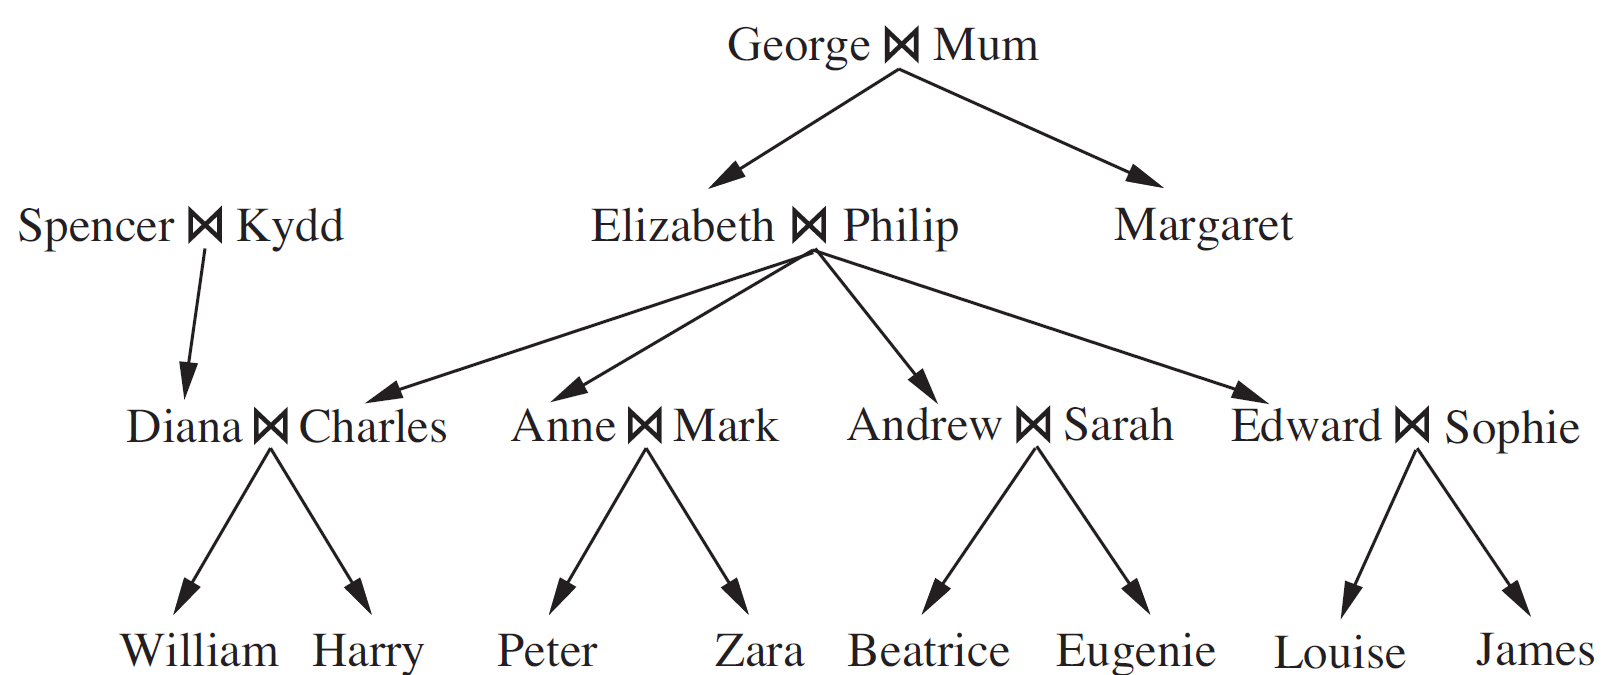
\includegraphics[width=15cm]{fig/family}

  \label{fig:family}
  \caption{A typical family tree. The symbol $\bowtie$ connects spouses and arrows point to children.}
\end{figure}
\begin{figure}[h]
  \centering
  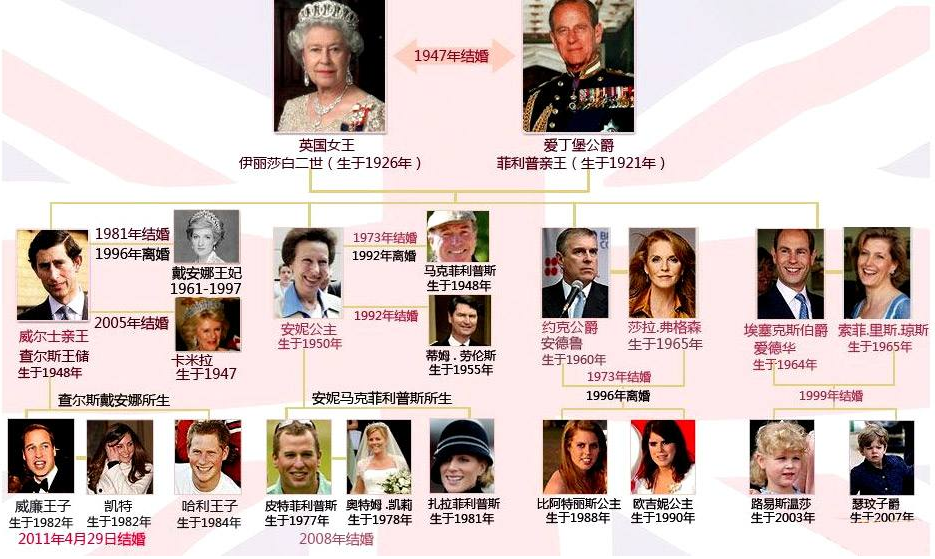
\includegraphics[width=15cm]{fig/Family_chinese.png}

  \label{fig:family_chinese}
  \caption{A typical family tree (Chinese version).}
\end{figure}

\section{Tasks}
\begin{enumerate}
\item Please complete the \texttt{Prolog} codes. There are several tutorials in the folder and I will explain the usage of Prolog in class.
\item Write the related codes and take a screenshot of the running results in the file named \textsf{E05\_YourNumber.pdf}, and send it to \textsf{ai\_201901@foxmail.com}.
\end{enumerate}

\section{Codes}
The Prolog code is very intuitive and reads as what it declares, but there are several things to mention.
\begin{itemize}
	\item Be careful of the possible values of \verb'X' and \verb'Y', since some rules may be satisfied when \verb'X=Y', which should have been eliminated.
	For example, \verb'sibling(X,Y)' needs to enforce constraint \verb'X \== Y', or \verb'X' and \verb'Y' may have the same parent, but they are also the same.
	\item \verb'firstCousin(X,Y)' not only needs to guarantee the grandparent of \verb'X' and \verb'Y' are the same, but also needs to make sure they do not have the same parent.
	\item The hardest part of this experiment is the design of the cousin logic.
	I firstly design an axillary function \verb'mthAncestor(X,Y,M)' for giving out the m-th ancestor \verb'Y' of \verb'X'.
	Notice the foundation part that \verb'M' is equal to zero, and it should return an identity function.
	\item Then I implement the \verb'mthCousin(X,Y,M)'.
	Many people only make \verb'X' and \verb'Y' have the same (m+1)-th ancestor \verb'Z' (the provided \verb'distance' function), which is not correct.
	Based on the definition of the m-th cousin, we should make sure \verb'X' and \verb'Y' get the same ancestor following different paths.
	Thus, the child of \verb'Z' on \verb'X''s path and the child of \verb'Z' on \verb'Y''s path should not be the same.
	So we have the constraints in Line 122.
	\item Finally is the \verb'mthCousinNremoved(X,Y,M,N)' rule which is similar to the implementation of the rule \verb'mthCousin'.
	The same ancestor \verb'Z' should have different children for \verb'X' and \verb'Y' to get up to there, as constrained in Line 126.
\end{itemize}
\begin{lstlisting}
/* facts */
oneself(george,george).
oneself(mum,mum).
oneself(spencer,spencer).
oneself(kydd,kydd).
oneself(elizabeth,elizabeth).
oneself(philip,philip).
oneself(margaret,margaret).
oneself(diana,diana).
oneself(charles,charles).
oneself(anne,anne).
oneself(mark,mark).
oneself(andrew,andrew).
oneself(sarah,sarah).
oneself(edward,edward).
oneself(sophie,sophie).
oneself(william,william).
oneself(harry,harry).
oneself(peter,peter).
oneself(zara,zara).
oneself(beatrice,beatrice).
oneself(eugenie,eugenie).
oneself(louise,louise).
oneself(james,james).

%% sex
% #1 gen
male(george).
female(mum).
% #2 gen
female(elizabeth).
male(philip).
female(margaret).
male(spencer).
female(kydd).
% #3 gen
female(diana).
male(charles).
female(anne).
male(mark).
male(andrew).
female(sarah).
male(edward).
female(sophie).
% #4 gen
male(william).
male(harry).
male(peter).
female(zara).
female(beatrice).
female(eugenie).
female(louise).
male(james).

%% parent
parent(diana,spencer).
parent(diana,kydd).
parent(william,diana).
parent(william,charles).
parent(harry,diana).
parent(harry,charles).
parent(charles,elizabeth).
parent(charles,philip).
parent(anne,elizabeth).
parent(anne,philip).
parent(peter,anne).
parent(peter,mark).
parent(zara,anne).
parent(zara,mark).
parent(andrew,elizabeth).
parent(andrew,philip).
parent(beatrice,andrew).
parent(beatrice,sarah).
parent(eugenie,andrew).
parent(eugenie,sarah).
parent(louise,edward).
parent(louise,sophie).
parent(james,edward).
parent(james,sophie).
parent(edward,elizabeth).
parent(edward,philip).
parent(elizabeth,george).
parent(elizabeth,mum).
parent(margaret,george).
parent(margaret,mum).

/* rules */
child(X,Y) :- parent(Y,X).
father(X,Y) :- parent(X,Y), male(Y).
mother(X,Y) :- parent(X,Y), female(Y).
husband(X,Y) :- female(X), male(Y), father(Z,Y), mother(Z,X).
wife(X,Y) :- male(X), female(Y), father(Z,X), mother(Z,Y).
spouse(X,Y) :- husband(X,Y) ; wife(X,Y).
son(X,Y) :- child(X,Y), male(Y).
daughter(X,Y) :- child(X,Y), female(Y).
sibling(X,Y) :- parent(X,Z), parent(Y,Z), X \== Y.
brother(X,Y) :- sibling(X,Y), male(Y).
sister(X,Y) :- sibling(X,Y), female(Y).
grandfather(X,Y) :- parent(X,Z), father(Z,Y).
grandmother(X,Y) :- parent(X,Z), mother(Z,Y).
grandchild(X,Y) :- child(X,Z), child(Z,Y).
grandparent(X,Y) :- parent(X,Z), parent(Z,Y).
greatGrandparent(X,Y) :- grandparent(X,Z), parent(Z,Y).
ancestor(X,Y) :- parent(X,Y). % Base
ancestor(X,Y) :- parent(X,Z), ancestor(Z,Y). % Recursion
aunt(X,Y) :- grandparent(X,Z), parent(Y,Z), \+(mother(X,Y)), female(Y).
uncle(X,Y) :- grandparent(X,Z), parent(Y,Z), \+(father(X,Y)), male(Y).
%% the husband of your sister or brother
%% or the brother of your husband or wife
%% or the man who is married to the sister
%% or brother of your wife or husband
brotherInLaw(X,Y) :- (spouse(X,Z), brother(Z,Y)) ; (sister(X,Z), husband(Z,Y)).
sisterInLaw(X,Y) :- (spouse(X,Z), sister(Z,Y)) ; (brother(X,Z), wife(Z,Y)).
% cousins
firstCousin(X,Y) :- grandparent(X,Z), grandparent(Y,Z), X \== Y, \+(sibling(X,Y)).
mthAncestor(X,Y,0) :- oneself(X,Y).
mthAncestor(X,Y,1) :- parent(X,Y).
mthAncestor(X,Y,M) :- parent(X,Z), M1 is M-1, mthAncestor(Z,Y,M1).
mthCousin(X,Y,1) :- firstCousin(X,Y).
mthCousin(X,Y,M) :-
	M1 is M+1, mthAncestor(X,Z,M1), mthAncestor(Y,Z,M1), X \== Y,
	mthAncestor(X,A,M), mthAncestor(Y,B,M), A \= B, parent(A,Z), parent(B,Z).
	%% mthAncestor(X,A,M), mthAncestor(Y,B,M), A \= B, \+(spouse(A,B)).
mthCousinNremoved(X,Y,M,N) :-
	M1 is M+1, mthAncestor(X,Z,M1), M2 is M-N+1, mthAncestor(Y,Z,M2), X \== Y,
	mthAncestor(X,A,M), M3 is M-N, mthAncestor(Y,B,M3), parent(A,Z), parent(B,Z), A \== B.
\end{lstlisting}

\section{Results}
The results are shown below, where I test all the cases in the questions.
\begin{figure}[H]
\centering
\begin{tabular}{c}
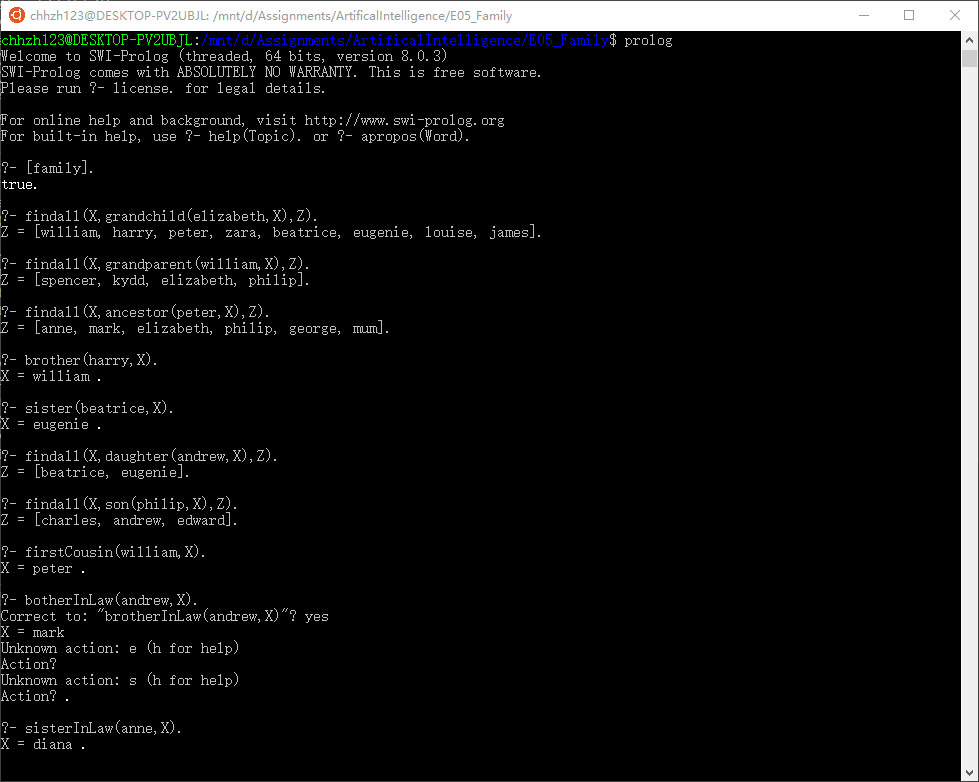
\includegraphics[width=\linewidth]{fig/result.png}\\
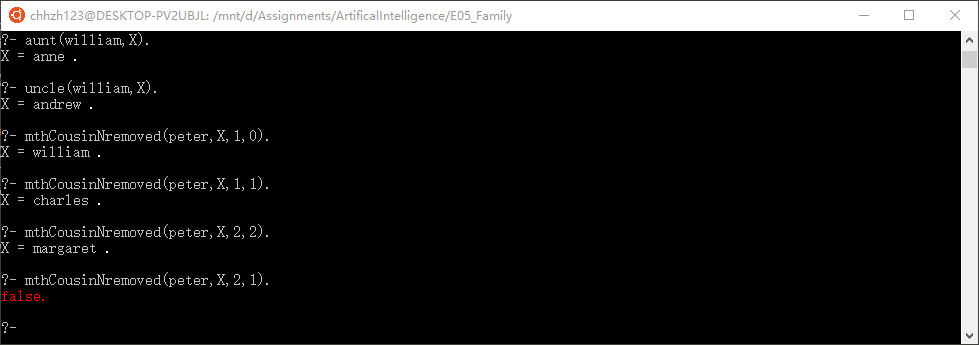
\includegraphics[width=\linewidth]{fig/result2.png}\\
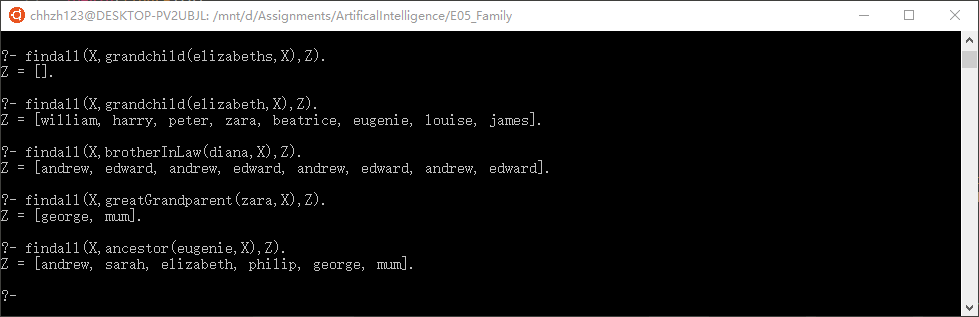
\includegraphics[width=\linewidth]{fig/result3.png}
\end{tabular}
\end{figure}

%\clearpage
%\bibliography{E:/Papers/LiuLab}
%\bibliographystyle{apalike}
\end{document}